\documentclass[aspectratio=169]{beamer}
%% Choose aspect ratio and other standard options:
[aspectratio=169] % 16:9 (default)
% [aspectratio=43]  % 4:3 

\hypersetup{pdfpagemode=FullScreen}

\usetheme[standard]{tugraz2018}
%% Choose main theme variant:
% [standard]        % standard (default)
% [institute]       % with institute's graphical acronym on the left
% [minimal]         % with reduced visuals

%% Choose your font style:
%                   % Helvetica (default for Corporate Design)
% [webfont]         % Source Sans Pro (as used on tugraz.at)
% [nofont]          % no font loaded - Computer Modern Sans

%% For more options, see README.pdf

\usepackage[utf8]{inputenc}
\usepackage[english]{babel}
%% Choose your main language:
% [ngerman]   % German
% [english]   % English


%% Add your own packages, macros, etc.
% ...


%% Enter presentation metadata
\title[AndroGUARD]{AndroGUARD: \\Implementing fingerprinting mitigation\\on Android}
\author{Gergö Kranz}
\date{05.07.2024}
\institute{IAIK}
\instituteurl{www.iaik.tugraz.at}

%% Logos
% \institutelogo{beamerthemetugraz/institute/kurz}  % graphical acronym for [institute] theme (left margin)
% \additionallogo{figures/logo}  % additional institute/department logo (footline; optional)
% \logobar{Supported by: ...}  % sponsors (titlepage; optional)


\begin{document}

\begin{frame}[plain]
  \maketitle
\end{frame}


\begin{frame}{Outline}
  \begin{minipage}{0.49\textwidth} 
    \tableofcontents
  \end{minipage}
  \hfill
  \begin{minipage}{0.49\textwidth} 
    \begin{figure}
      \centering
      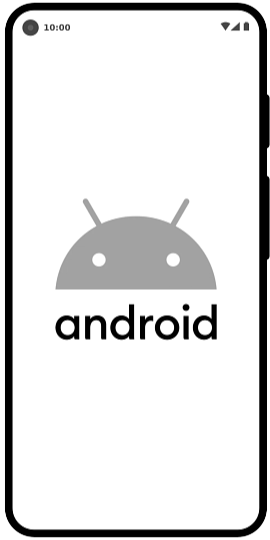
\includegraphics[height=0.5\textheight]{figures/android_device.png}
    \end{figure}
  \end{minipage}
\end{frame}


\section{Motivation}

\begin{frame}{Motivation}
  \hfill \hfill \hfill \hfill \hfill \hfill \hfill
  \begin{figure}
    \centering
    
\includegraphics[width=\textwidth]{figures/eyes.png}
  \end{figure}
\end{frame}


\section{Fingerprinting}

\begin{frame}{How does Fingerprinting work}
  \begin{minipage}{0.49\textwidth} 
    \begin{itemize}
      \item Extract information about the system
      \pause
      \item Analyse extracted information
      \pause
      \item Combine unique values into a unique identifier
    \end{itemize}
  \end{minipage}
  \hfill
  \begin{minipage}{0.49\textwidth} 
    \begin{figure}
      \centering
      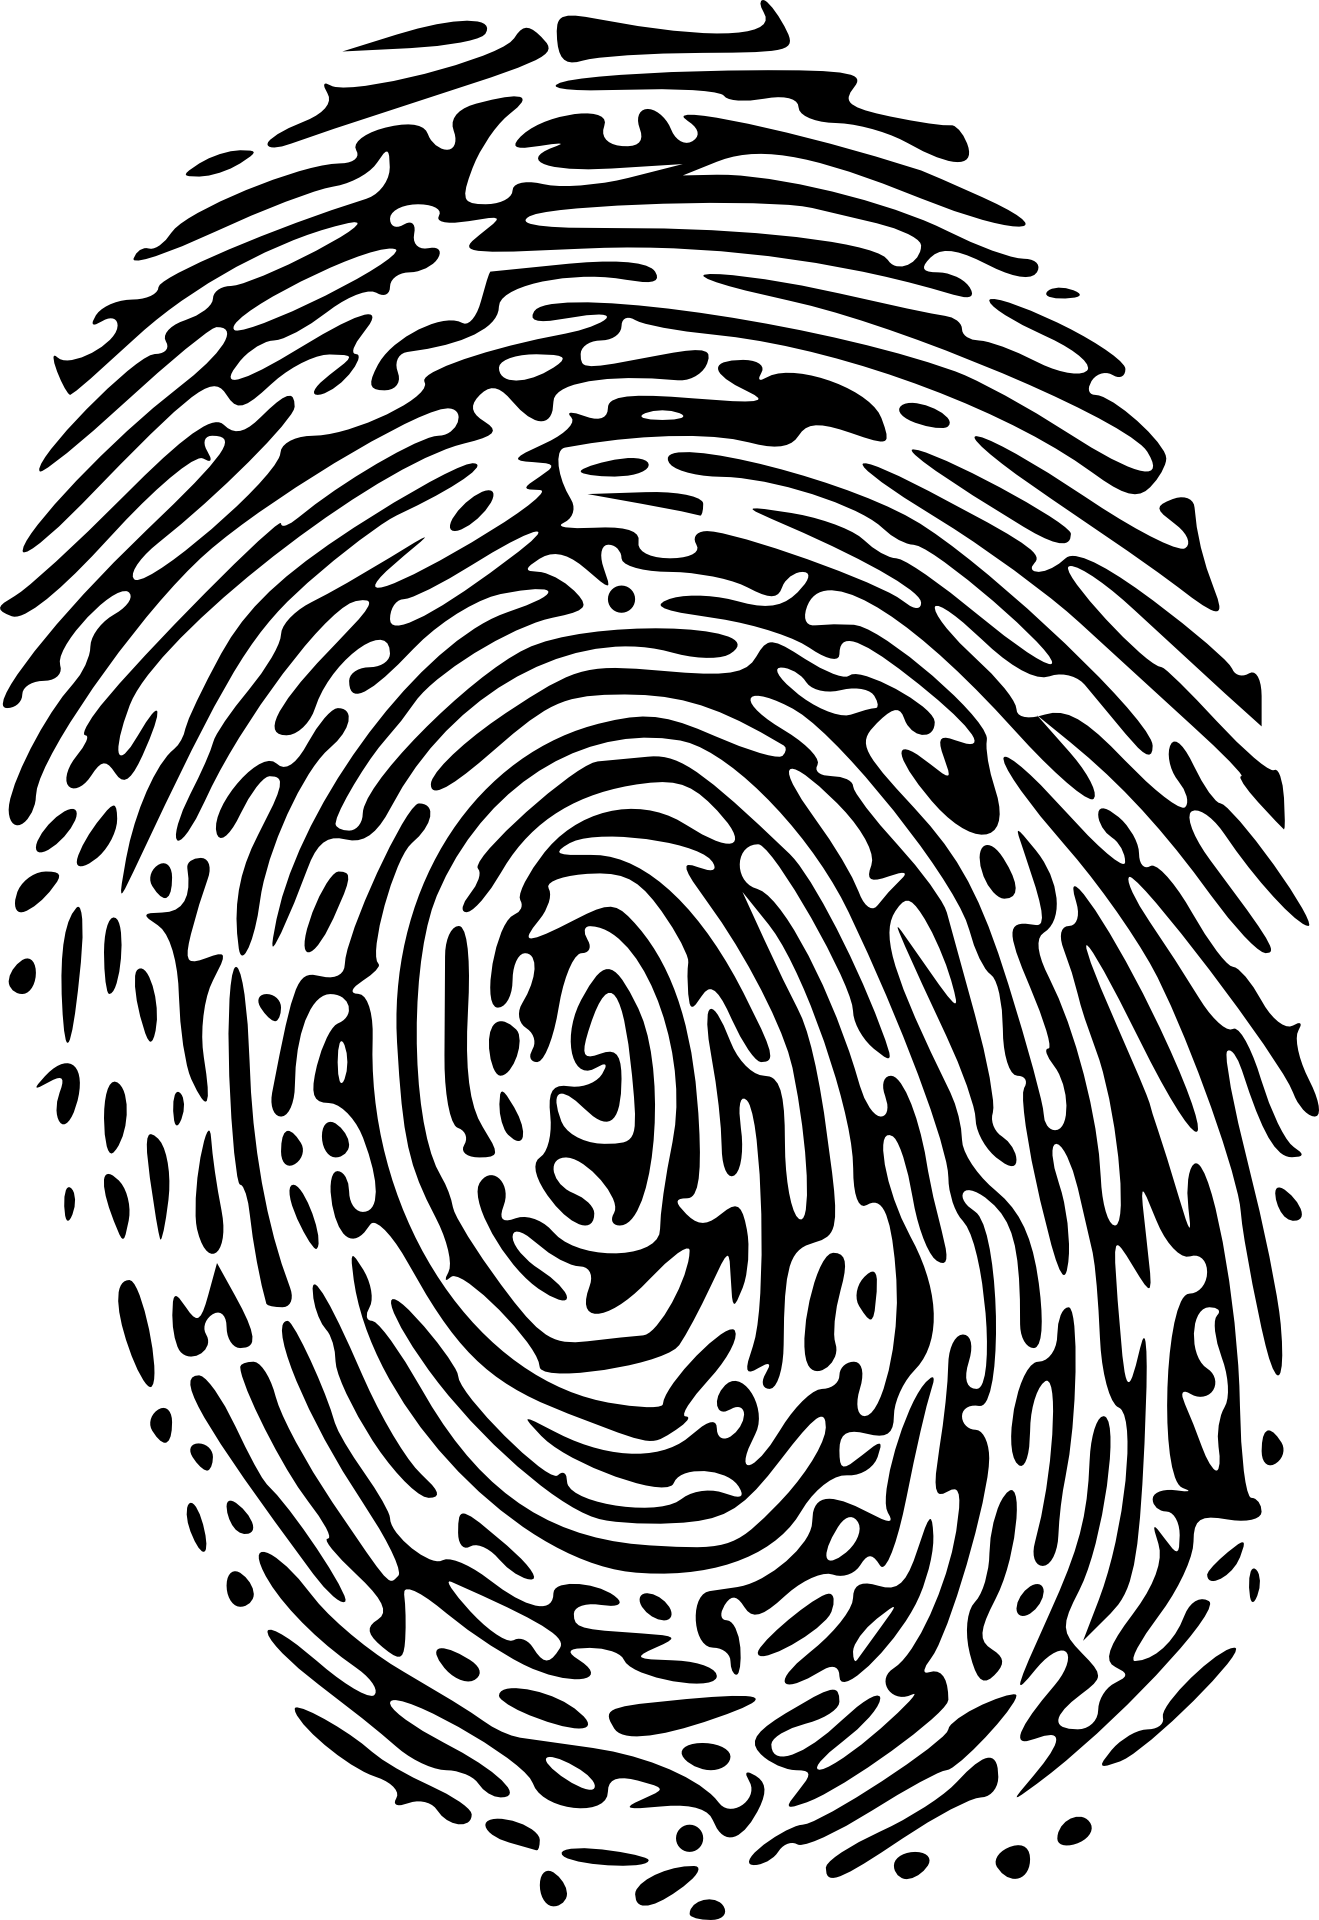
\includegraphics[height=0.5\textheight]{figures/fingerprint.png}
    \end{figure}
  \end{minipage}
\end{frame}

\begin{frame}{Fingerprinting Sensors}
  \begin{minipage}{0.49\textwidth} 
    \begin{itemize}
      \item Builtin Error
      \item Is consistent over the lifetime of the sensor
      \item Hardware can be uniquely identified
    \end{itemize}
  \end{minipage}
  \hfill
  \begin{minipage}{0.49\textwidth} 
    \begin{figure}
      \centering
      
\includegraphics[height=0.5\textheight]{figures/machine.png}
    \end{figure}
  \end{minipage}
\end{frame}

\begin{frame}{Fingerprinting Sensors}
  \begin{minipage}{0.49\textwidth} 
    \begin{itemize}
      \item Records multiple measurements
      \item Calculates the deviation from expected values
    \end{itemize}
  \end{minipage}
  \hfill
  \begin{minipage}{0.49\textwidth} 
    \begin{figure}
      \centering
      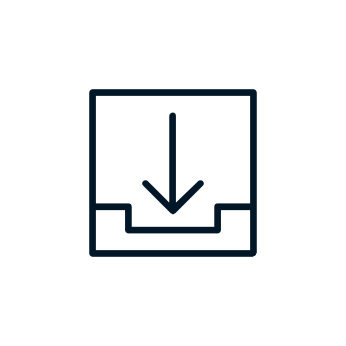
\includegraphics[height=0.5\textheight]{figures/download.png}
    \end{figure}
  \end{minipage}
\end{frame}

\section{Main Question}

\begin{frame}{Main Question}
  \begin{minipage}{0.525\textwidth} 
    How to protect against fingerprinting
  \end{minipage}
  \hfill
  \begin{minipage}{0.455\textwidth} 
    \begin{figure}
      \centering
      
\includegraphics[height=0.5\textheight]{figures/question.png}
    \end{figure}
  \end{minipage}
\end{frame}

\section{Background on existing work}

\begin{frame}{Existing Methods}
  \begin{minipage}{0.49\textwidth} 
    \begin{itemize}
      \item Access Control
    \end{itemize}
  \end{minipage}
  \hfill
  \begin{minipage}{0.49\textwidth} 
    \begin{figure}
      \centering
      
\includegraphics[height=0.5\textheight]{figures/android.png}
    \end{figure}
  \end{minipage}
\end{frame}

\begin{frame}{Related Works}
  \begin{minipage}{0.49\textwidth} 
    \begin{itemize}
      \item Many papers are looking into exploiting sensor fingerprinting
      \pause
      \item Do not implement a solution for the Android API
    \end{itemize}
  \end{minipage}
  \hfill
  \begin{minipage}{0.49\textwidth} 
    \begin{figure}
      \centering
      
\includegraphics[height=0.5\textheight]{figures/paper.png}
    \end{figure}
  \end{minipage}
\end{frame}

\begin{frame}{Proposed Solutions}
  \begin{minipage}{0.49\textwidth} 
    \begin{itemize}
      \item Recalibrate the sensors to be perfect
      \begin{itemize}
        \item Gets rid of the error
        \item Can not be done easily
      \end{itemize}
    \end{itemize}
  \end{minipage}
  \hfill
  \begin{minipage}{0.49\textwidth} 
    \begin{figure}
      \centering
      
\includegraphics[height=0.5\textheight]{figures/tool.png}
    \end{figure}
  \end{minipage}
\end{frame}

\begin{frame}{Proposed Solutions}
  \begin{minipage}{0.49\textwidth} 
    \begin{itemize}
      \item Add noise to conceal the calibration errors
      \begin{itemize}
        \item Apply a random offset and gain to each measurement
        \item Can be done without any user interaction
      \end{itemize}
    \end{itemize}
  \end{minipage}
  \hfill
  \begin{minipage}{0.49\textwidth} 
    \begin{figure}
      \centering
      
\includegraphics[height=0.5\textheight]{figures/noise.png}
    \end{figure}
  \end{minipage}
\end{frame}

\section{Our Approach}

\begin{frame}{Protecting Sensors}
  \begin{minipage}{0.49\textwidth} 
    \begin{itemize}
      \item Mask builtin error by added noise
      \pause
      \item Use the A2P2 framework for deployment
    \end{itemize}
  \end{minipage}
  \hfill
  \begin{minipage}{0.49\textwidth} 
    \begin{figure}
      \centering
      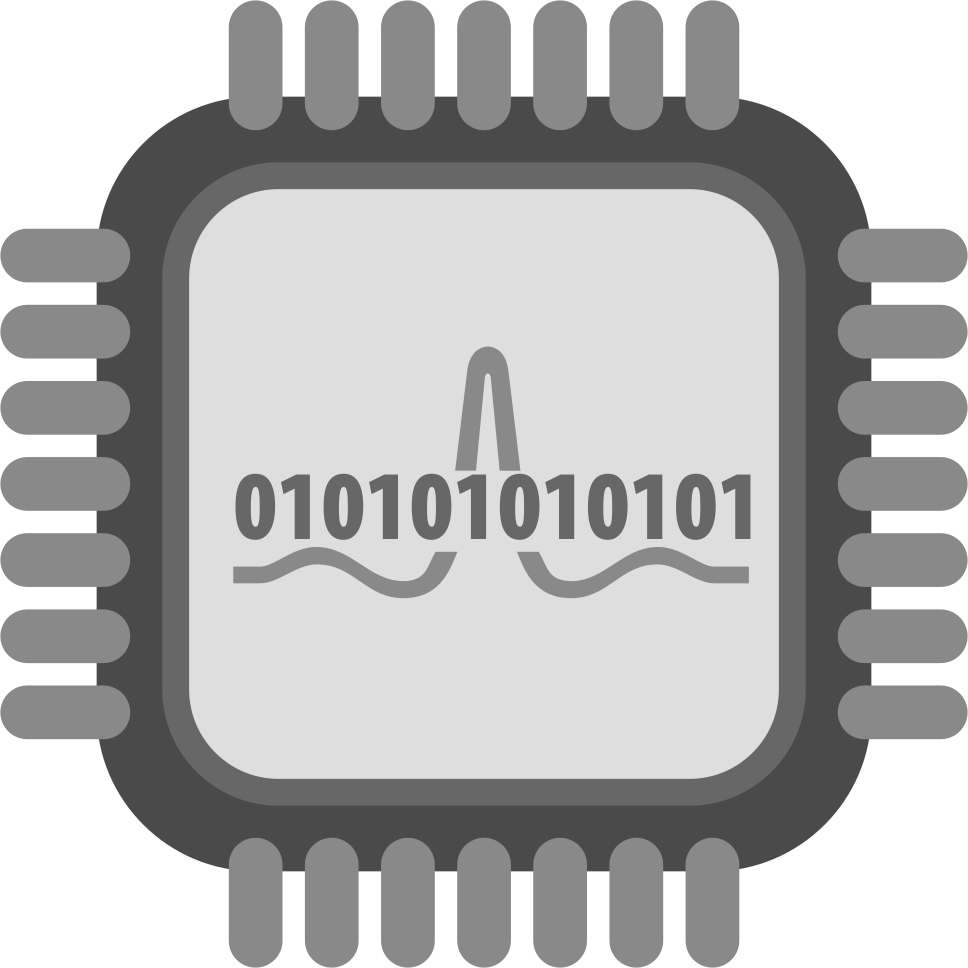
\includegraphics[height=0.5\textheight]{figures/analog.png}
    \end{figure}
  \end{minipage}
\end{frame}

\begin{frame}{Implementation}
  \begin{minipage}{0.49\textwidth} 
    \begin{itemize}
      \item Intercept the original method
      \pause
      \item Apply appropriate random noise
      \pause
      \item Return obstructed sensor data to original method
    \end{itemize}
  \end{minipage}
  \hfill
  \begin{minipage}{0.49\textwidth} 
    \begin{figure}
      \centering
      
\includegraphics[height=0.5\textheight]{figures/java.png}
    \end{figure}
  \end{minipage}
\end{frame}

\section{Deployment}

\begin{frame}{A2P2}
  \begin{minipage}{0.49\textwidth} 
    \begin{itemize}
      \item Incorporates the patch into a valid APK
      \item Intercepts the original function calls
      \item Executes the patch
    \end{itemize}
  \end{minipage}
  \hfill
  \begin{minipage}{0.49\textwidth} 
    \begin{figure}
      \centering
      
\includegraphics[height=0.5\textheight]{figures/code.png}
    \end{figure}
  \end{minipage}
\end{frame}

\section{Validation}

\begin{frame}{Validation}
  \begin{minipage}{0.49\textwidth} 
    \begin{itemize}
      \item Comparing values before and after the patch
      \item Could not be done sufficiently due to limited access to supported hardware
    \end{itemize}
  \end{minipage}
  \hfill
  \begin{minipage}{0.49\textwidth} 
    \begin{figure}
      \centering
      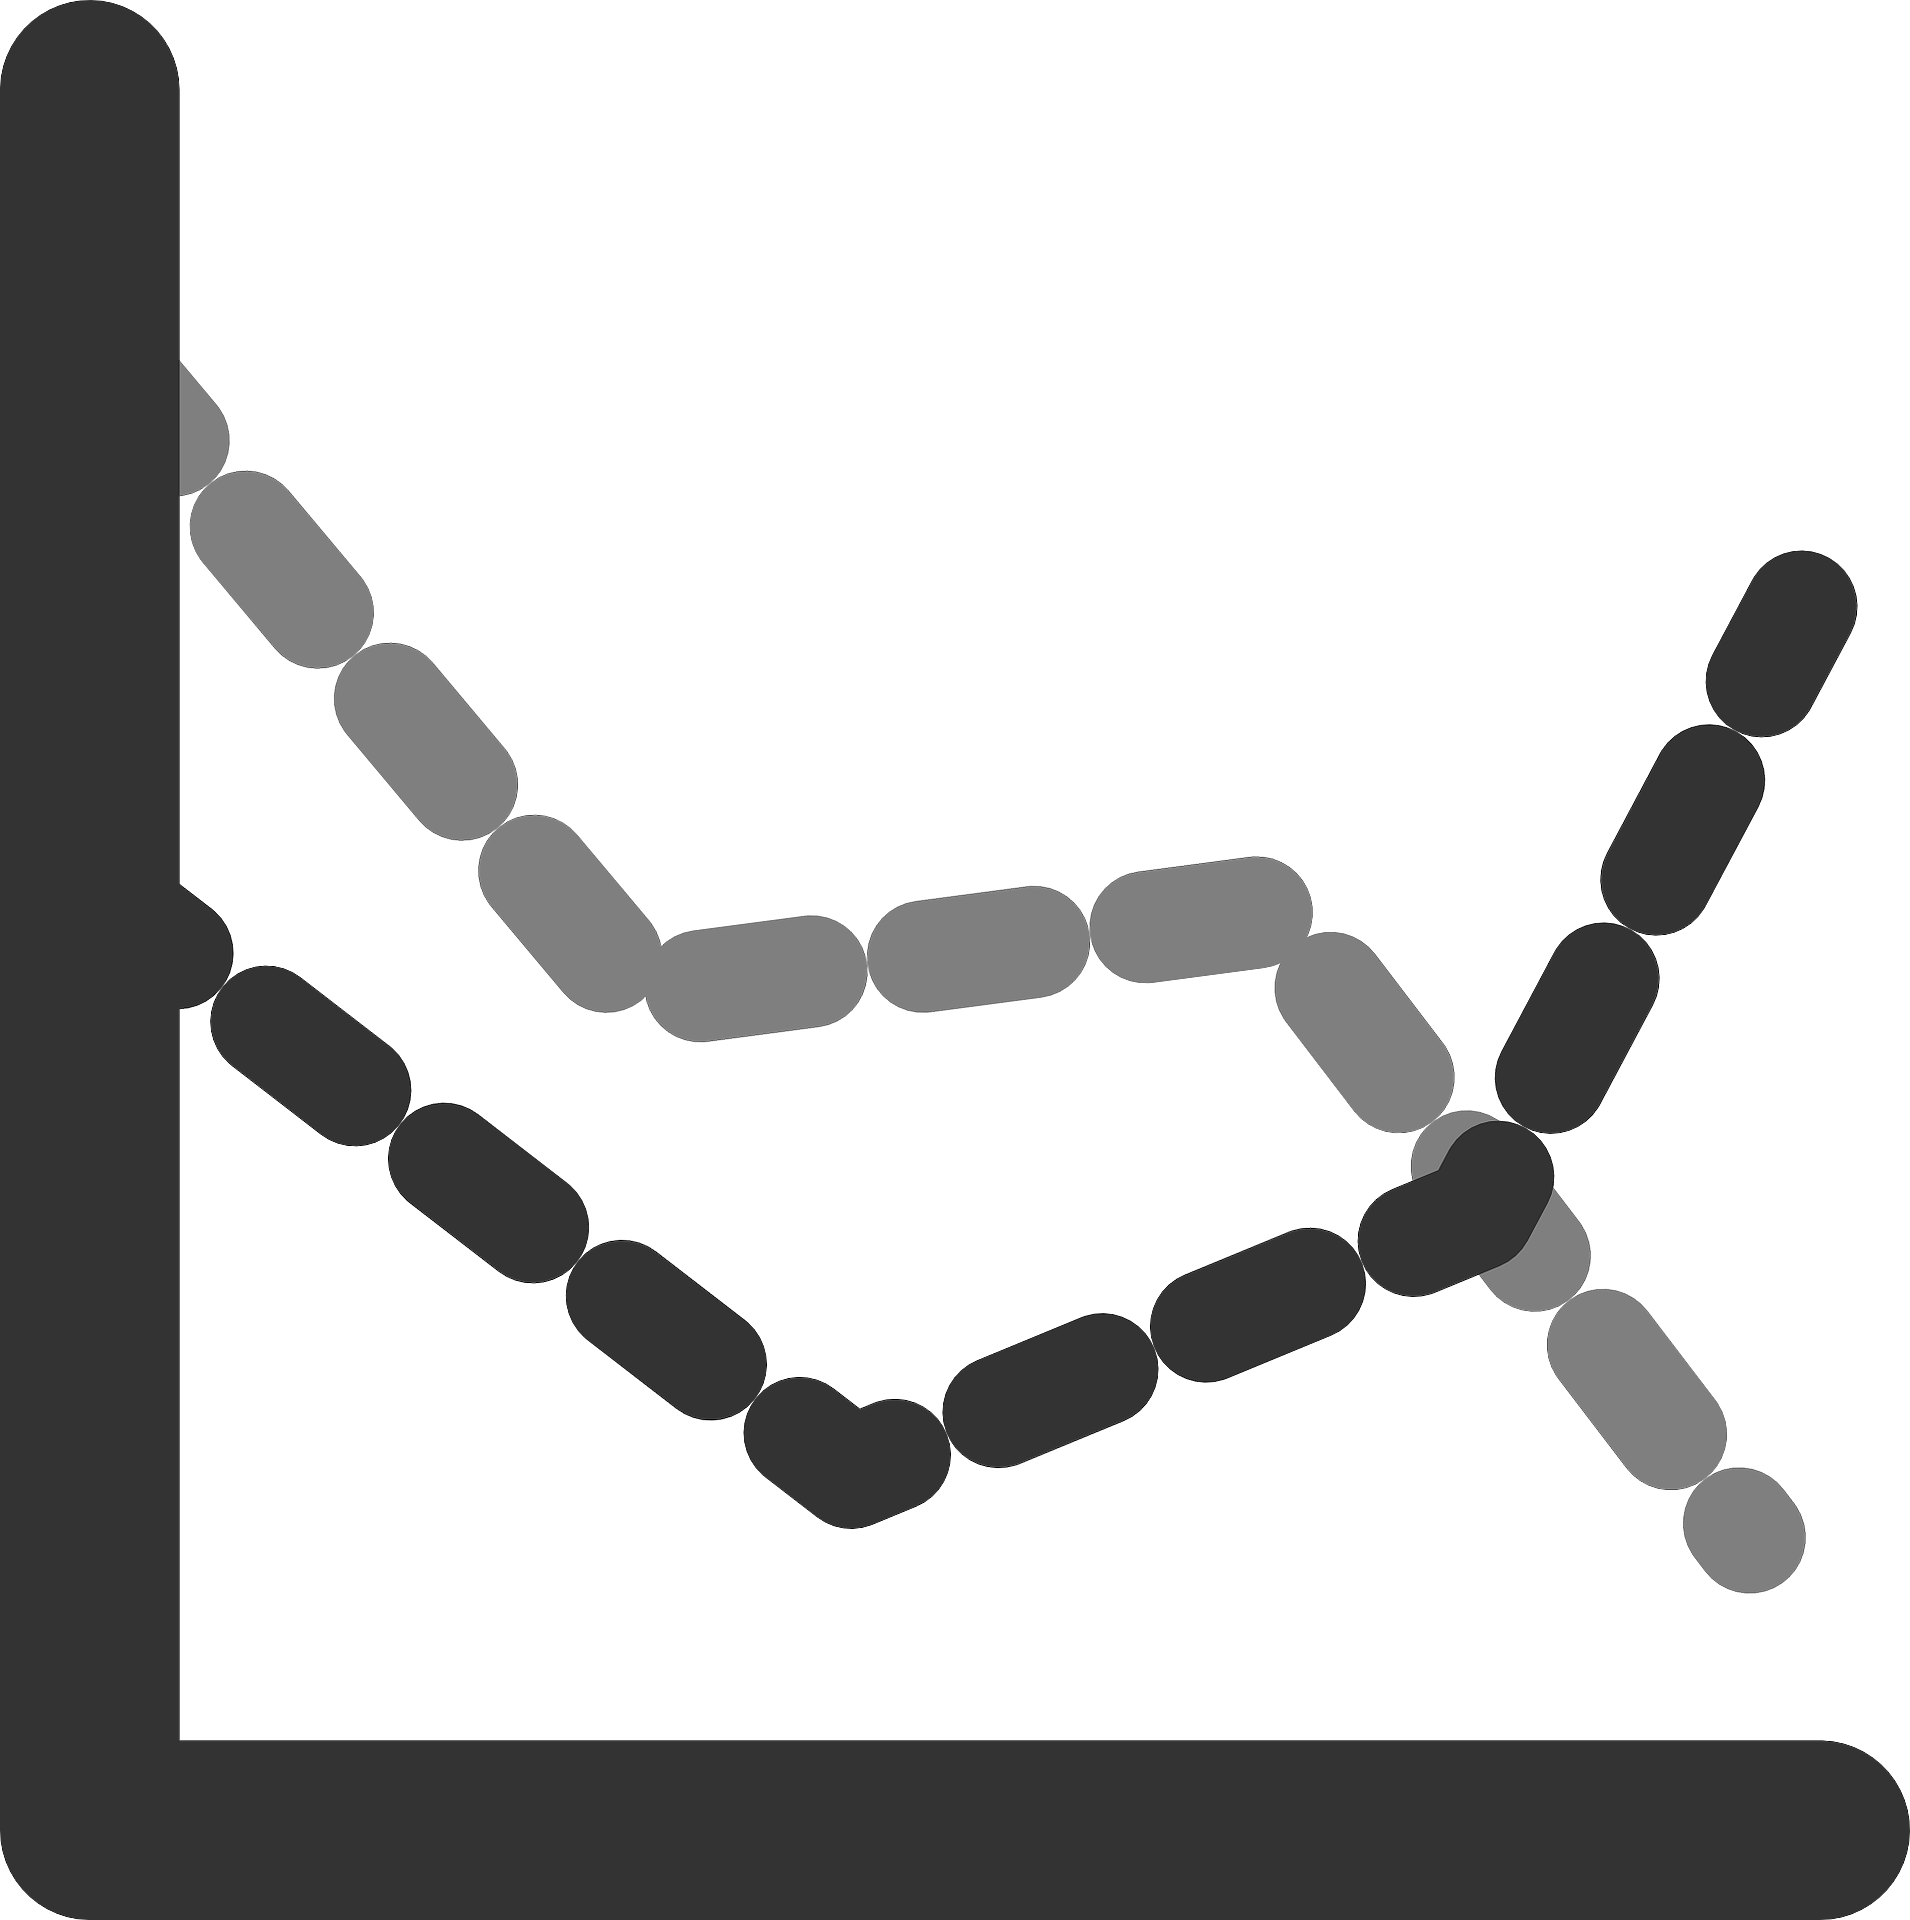
\includegraphics[height=0.5\textheight]{figures/graph.png}
    \end{figure}
  \end{minipage}
\end{frame}

\section*{}

\begin{frame}{Conclusion}
  \begin{minipage}{0.49\textwidth} 
    \begin{itemize}
      \item Masking the sensor values decreases fingerprintability
      \item Modifying the SensorEventListener makes it easy to incorporate the patch into the Android API
    \end{itemize}
  \end{minipage}
  \hfill
  \begin{minipage}{0.49\textwidth} 
    \begin{figure}
      \centering
      
\includegraphics[height=0.5\textheight]{figures/androguard.png}
    \end{figure}
  \end{minipage}
\end{frame}


% \begin{frame}{Bibliography}
%   ...
% \end{frame}

\end{document}
